% Les annexes contiennent généralement :

% \begin{itemize}
%     \item les dessins mécaniques (mises en plan);
%     \item les schémas électriques détaillés;
%     \item des photographies du projet;
%     \item des scripts et des extraits de code source;
%     \item des documents techniques \pex \emph{datasheet};
%     \item des développements mathématiques.
% \end{itemize}
\newpage
\section*{Mises en plan} \label{Mises_En_Plan}
\addcontentsline{toc}{section}{Mises en plan}
\begin{figure}[H]
    \centering
    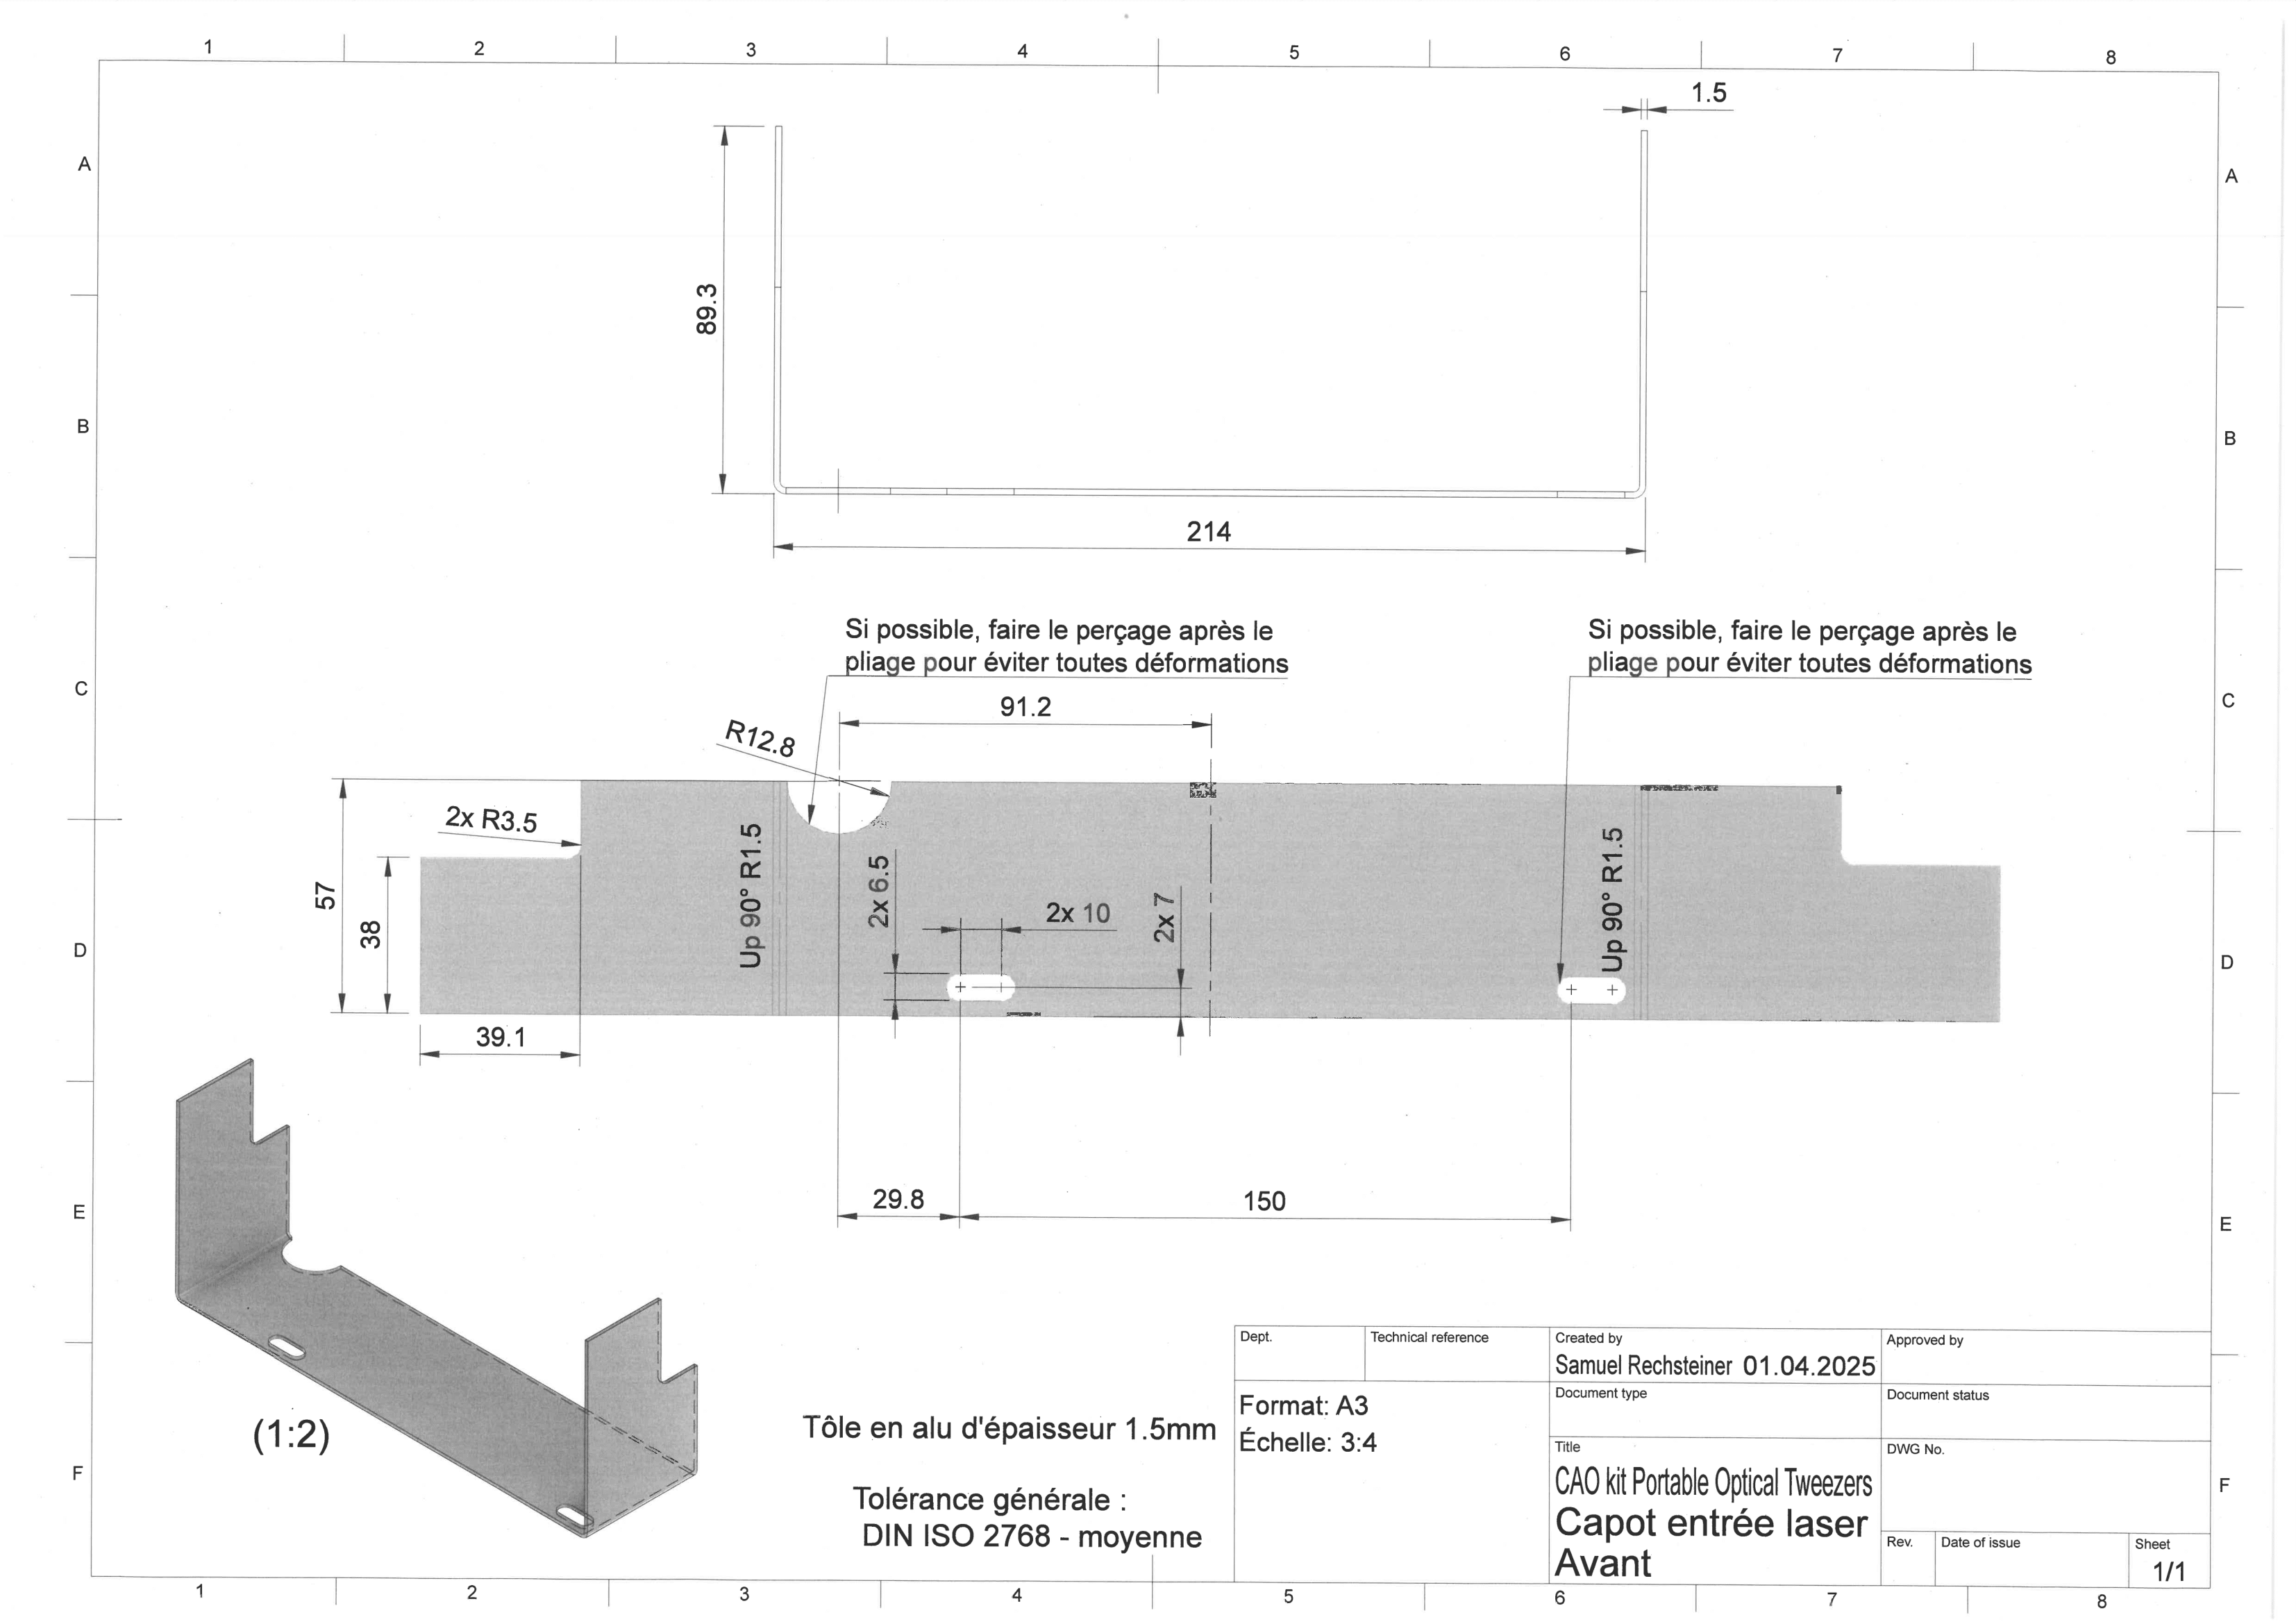
\includegraphics[angle=90,width=\textwidth]{assets/figures/Annexes/Mises_en_plan/mise_en_plan_avant.png}
    \caption{Mise en plan du capot inférieur avant}
    \label{mise_en_plan_capot_avant}
\end{figure}

\begin{figure}[H]
    \centering
    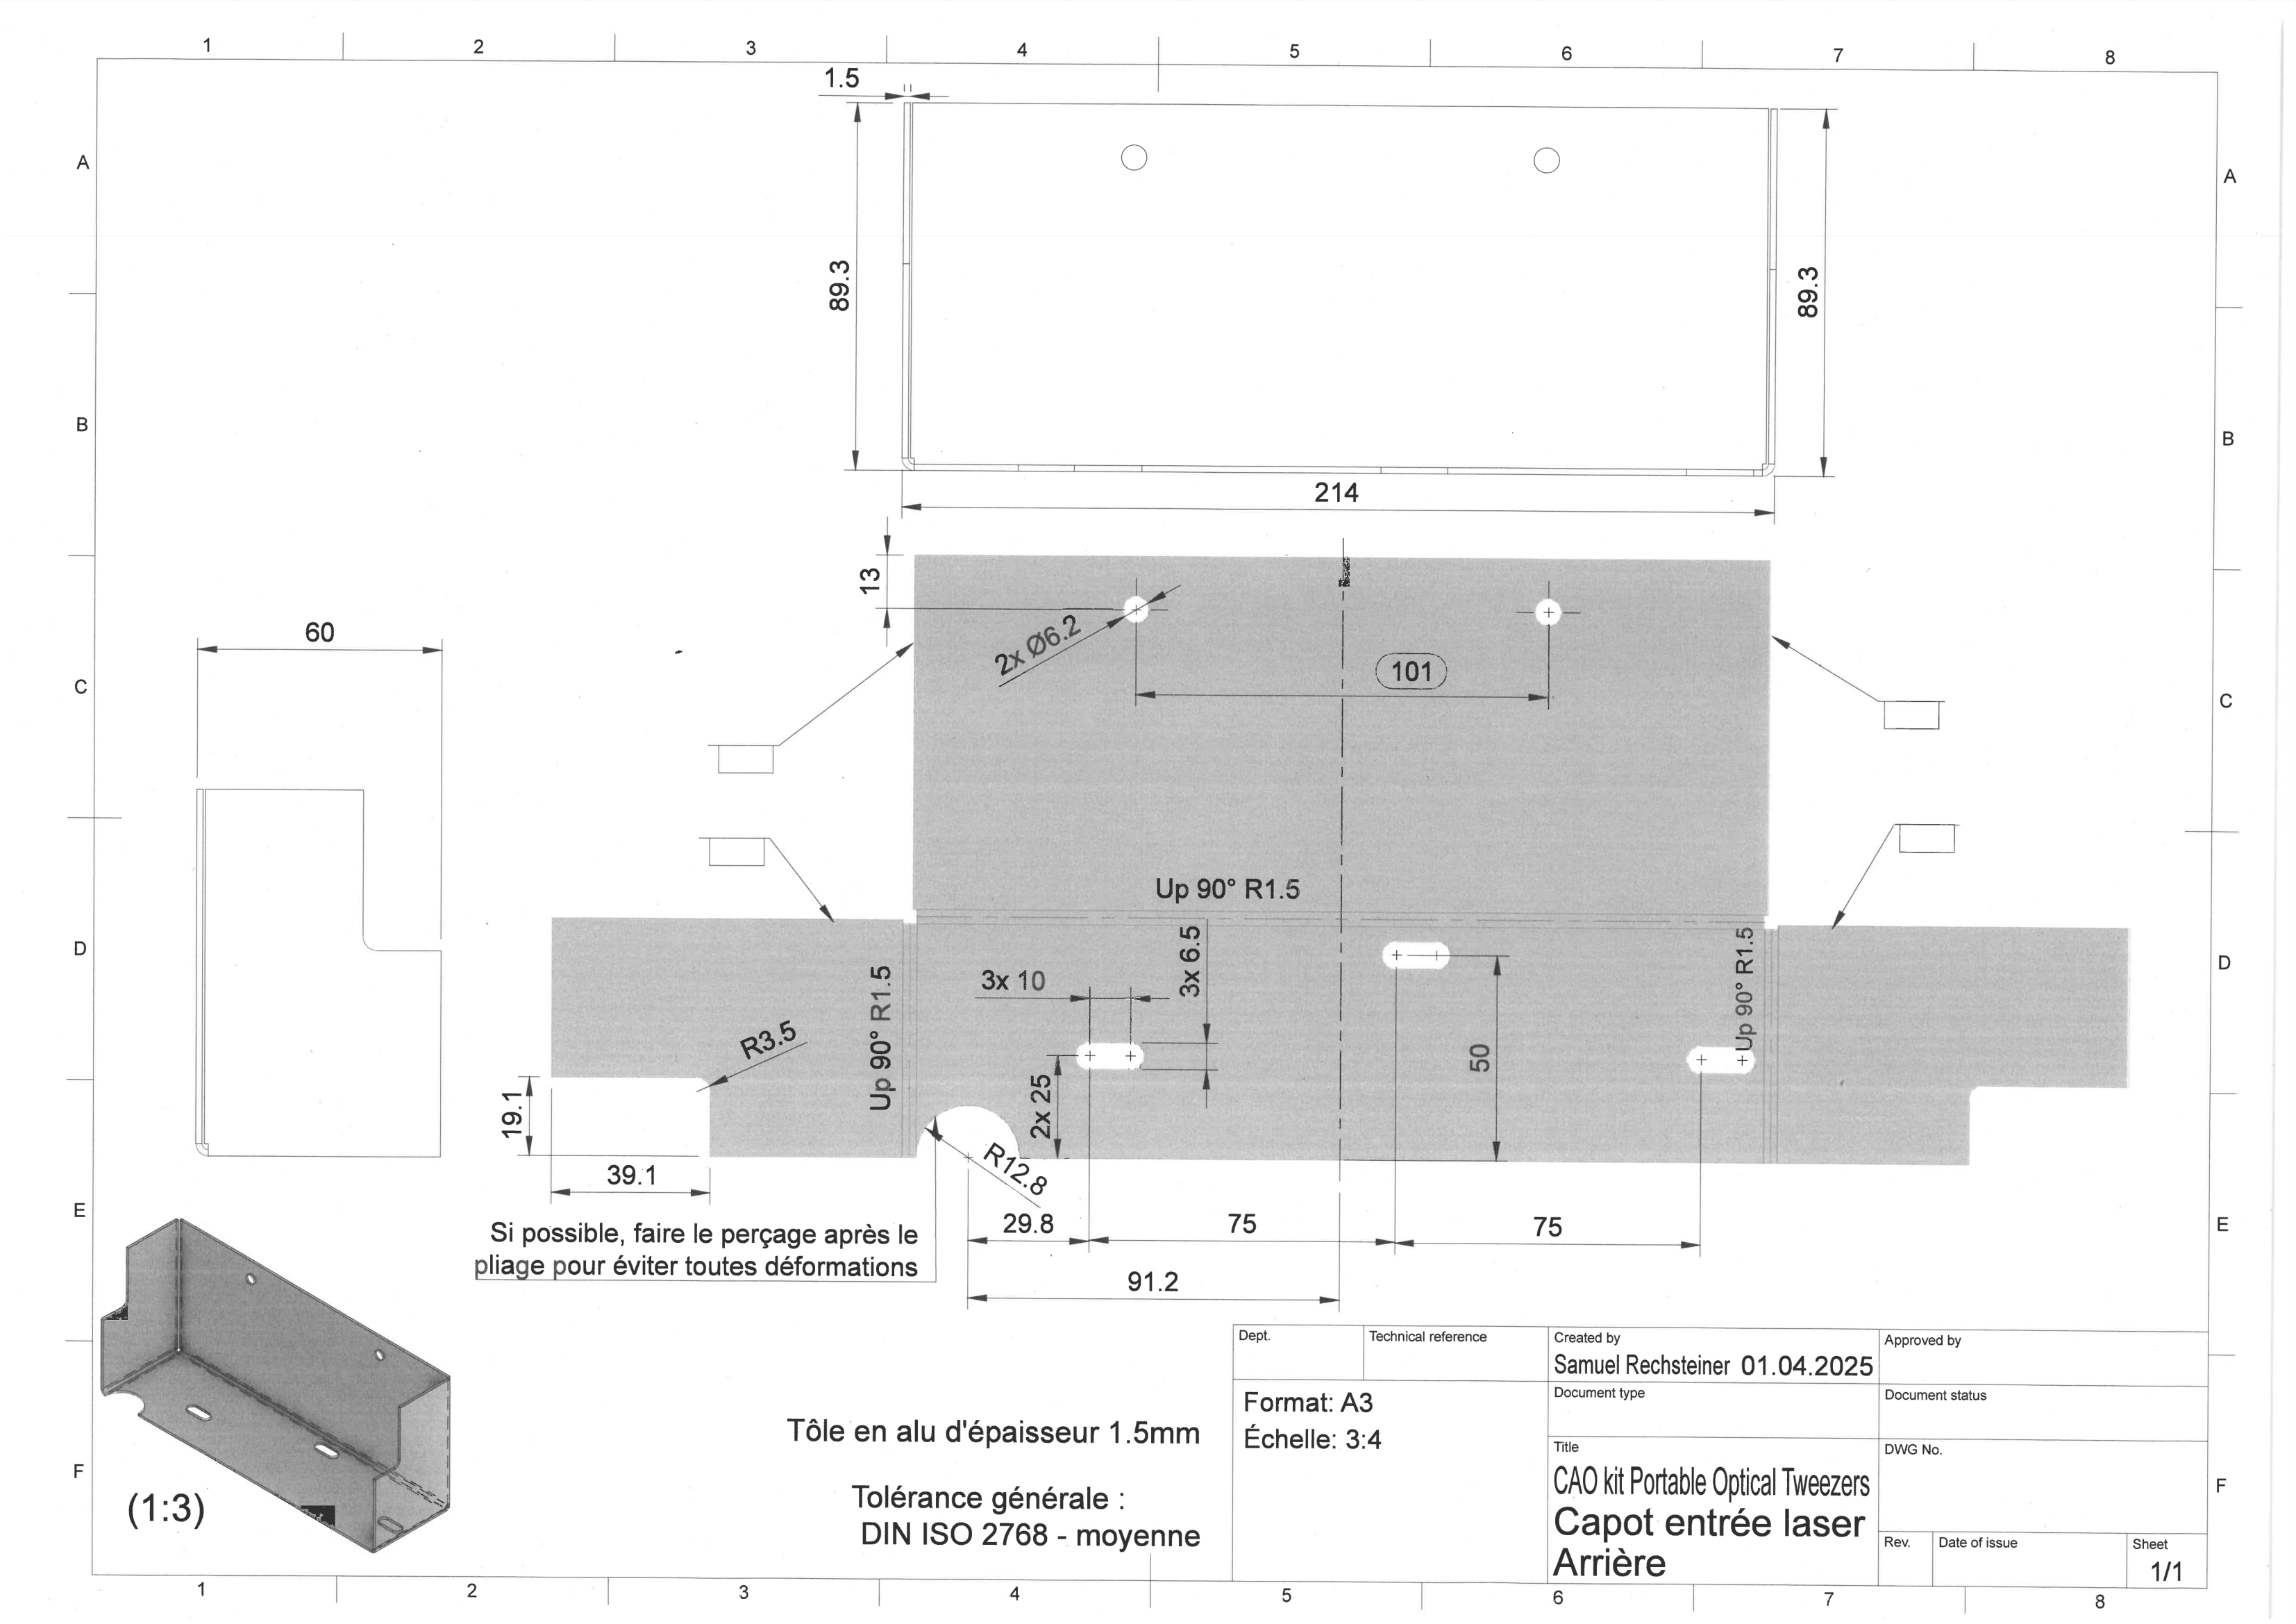
\includegraphics[angle=90,width=\textwidth]{assets/figures/Annexes/Mises_en_plan/mise_en_plan_arriere.png}
    \caption{Mise en plan du capot inférieur arrière}
    \label{mise_en_plan_capot_arriere}
\end{figure}

\begin{figure}[H]
    \centering
    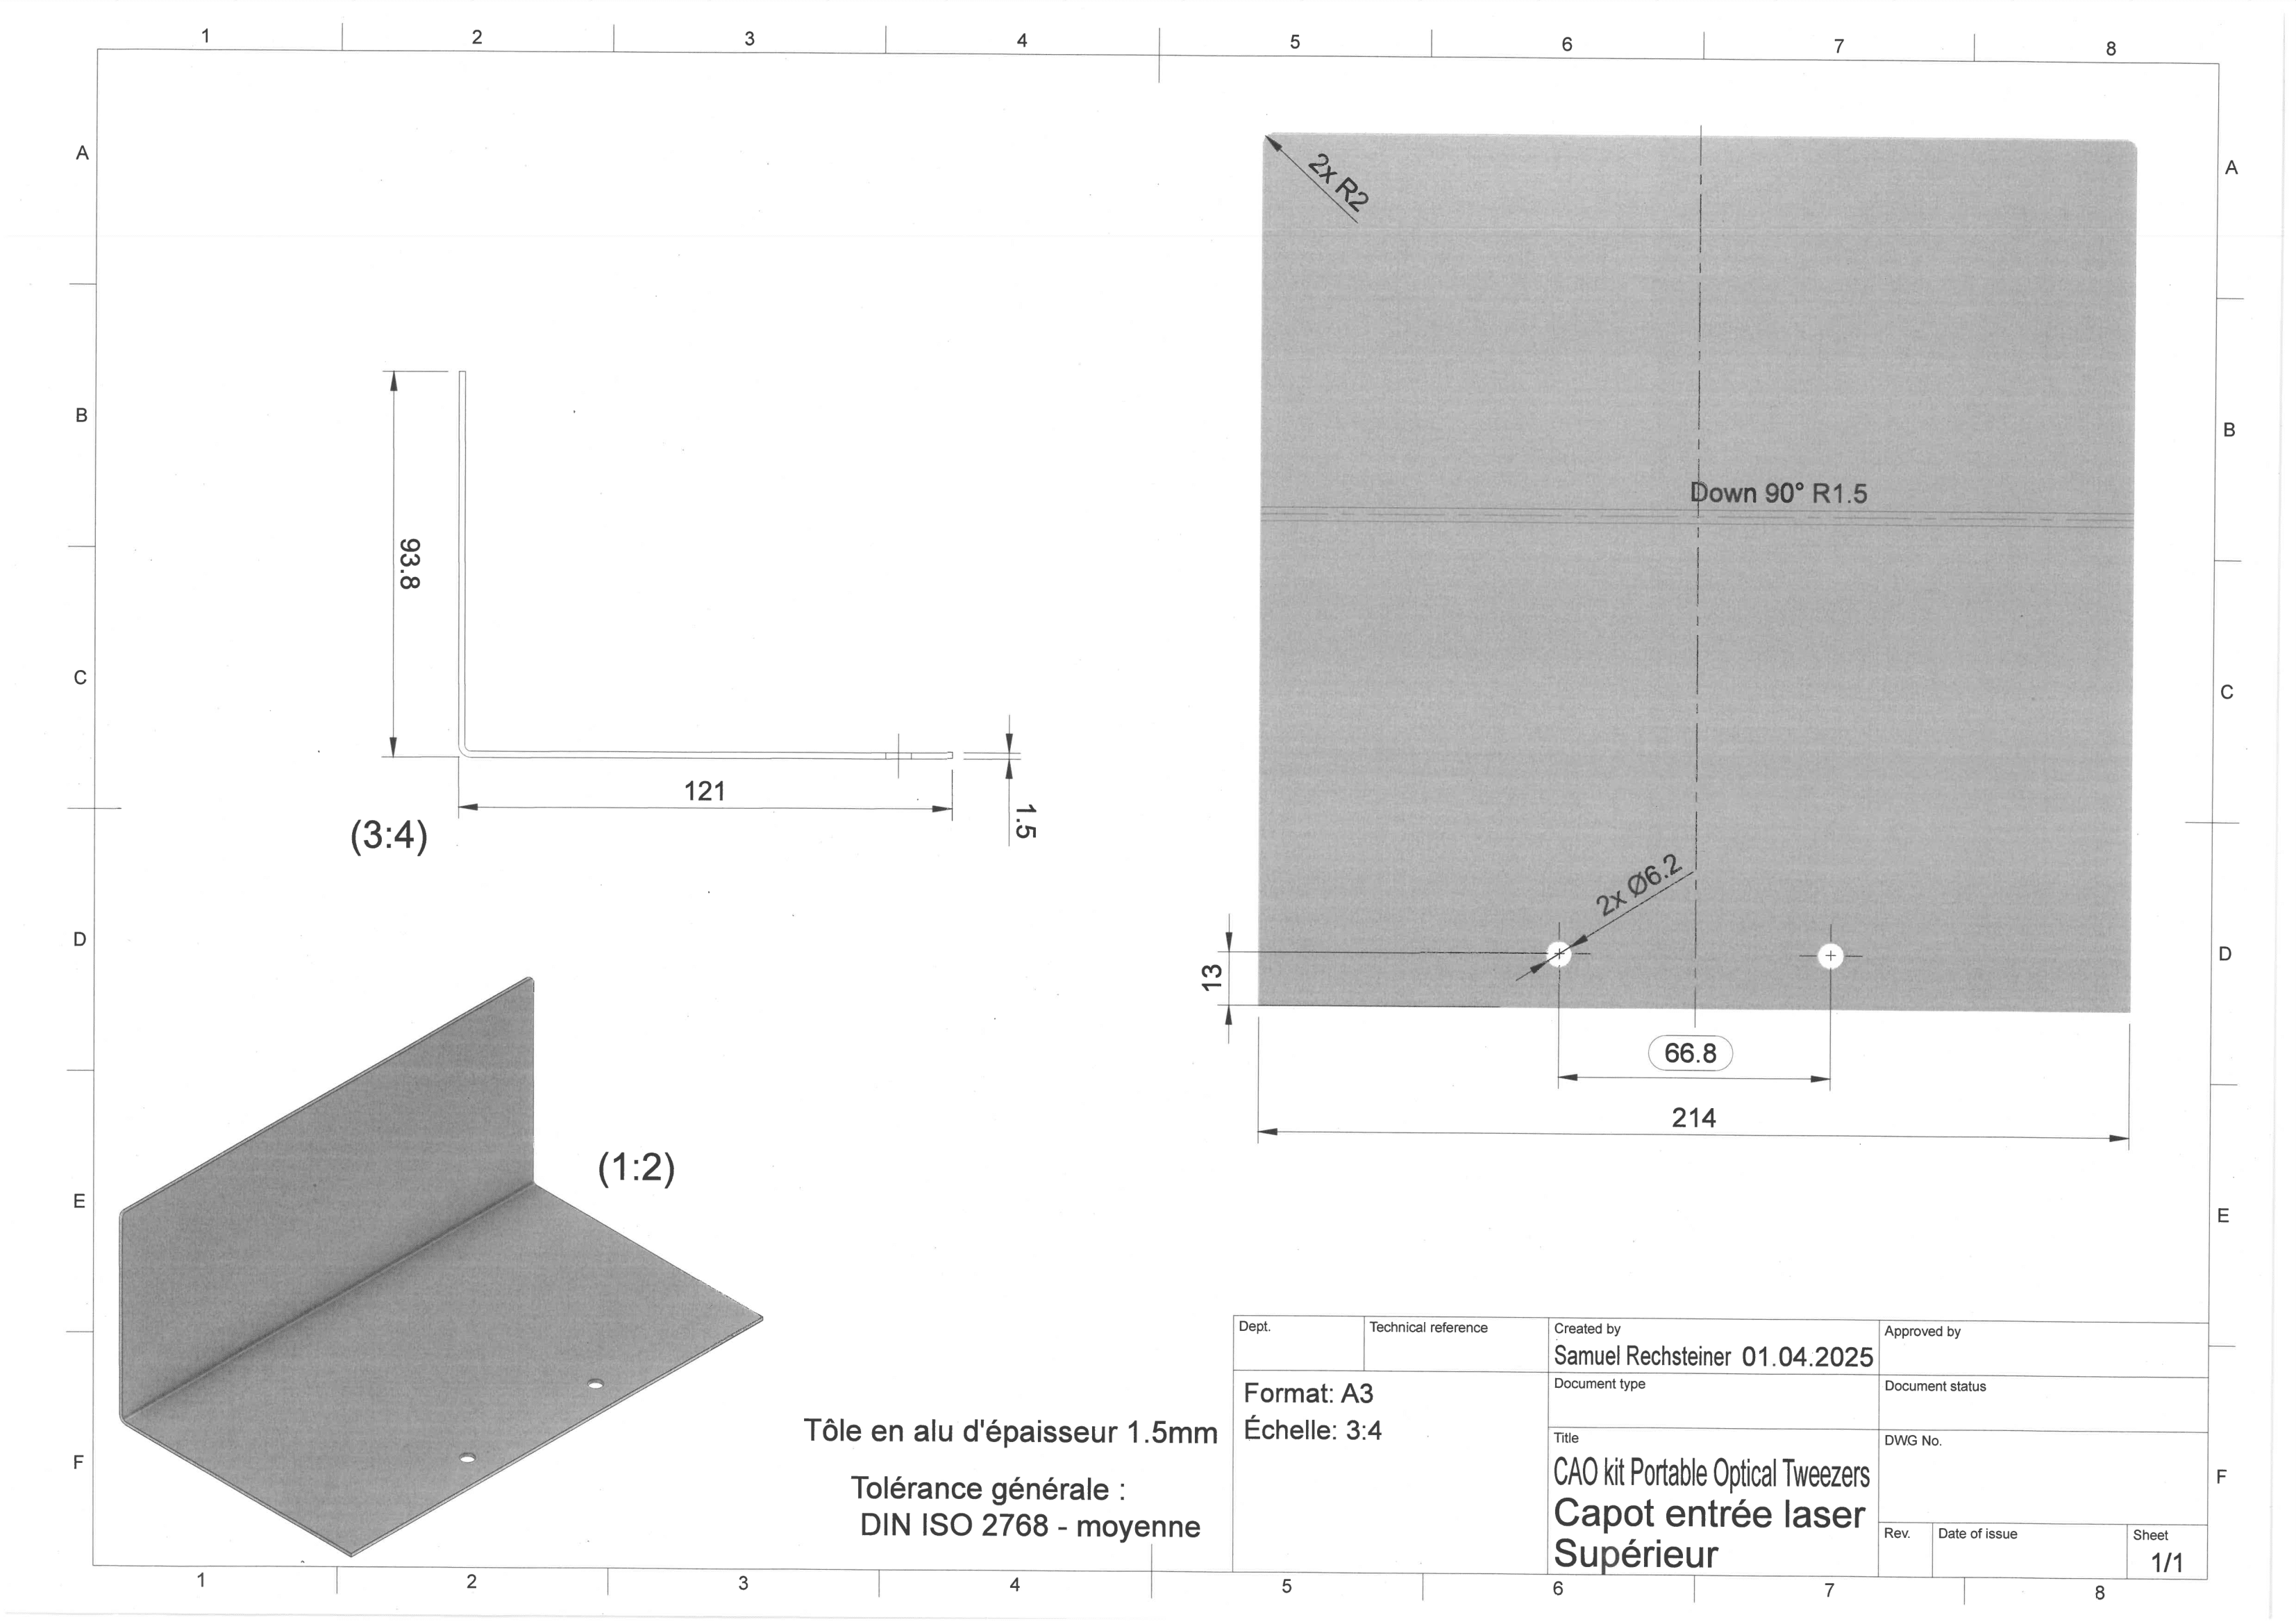
\includegraphics[angle=90,width=\textwidth]{assets/figures/Annexes/Mises_en_plan/mise_en_plan_superieur.png}
    \caption{Mise en plan du capot supérieur}
    \label{mise_en_plan_capot_superieur}
\end{figure}

\clearpage
\section*{Notice de laboratoire pour Kinesis \& ThorCam} \label{annexe:notice_labo_Kinesis_ThorCam}
\addcontentsline{toc}{section}{Notice de laboratoire pour Kinesis \& ThorCam}
\includepdf[pages=-,pagecommand={},width=1.2\textwidth]{assets/figures/Annexes/Notice_labo_Portable_Optical_Tweezers_Kinesis_ThorCam.pdf}

\section*{Notice de laboratoire pour ServoVision} \label{annexe:notice_labo_ServoVision}
\addcontentsline{toc}{section}{Notice de laboratoire pour ServoVision}
\includepdf[pages=-,pagecommand={},width=1.2\textwidth]{assets/figures/Annexes/Notice_labo_Portable_Optical_Tweezers_ServoVision.pdf}